\documentclass[11pt,letterpaper]{article}
\usepackage[T1]{fontenc}
\usepackage[utf8]{inputenc}
\usepackage{mathptmx}
\usepackage[margin=2.2cm]{geometry}
\usepackage{graphicx,xcolor,booktabs,amsmath,amssymb,siunitx,tikz,caption,subcaption,hyperref,fancyhdr,float,listings}
\lstset{language=Python,columns=fullflexible,keepspaces=true,basicstyle=\ttfamily\scriptsize,keywordstyle=\color{blue!60!black}\bfseries,commentstyle=\color{green!40!black}\itshape,stringstyle=\color{red!50!black},numbers=left,numberstyle=\tiny\color{gray},frame=single,breaklines=true,showstringspaces=false,backgroundcolor=\color{gray!5},inputencoding=utf8,extendedchars=true,literate={á}{{\'a}}1 {é}{{\'e}}1 {í}{{\'i}}1 {ó}{{\'o}}1 {ú}{{\'u}}1 {ñ}{{\~n}}1 {°}{{$^\circ$}}1 {δ}{{$\delta$}}1 {η}{{$\eta$}}1 {√}{{$\surd$}}1 {²}{{$^2$}}1 {≈}{{$\approx$}}1 {→}{{$\to$}}1 {Δ}{{$\Delta$}}1}
\renewcommand{\lstlistingname}{Código}
\hypersetup{colorlinks=true,linkcolor=blue!50!black,citecolor=blue!50!black,urlcolor=blue!50!black}
\renewcommand{\figurename}{Figura}\renewcommand{\tablename}{Tabla}\renewcommand{\refname}{Referencias}\renewcommand{\abstractname}{Resumen}
\captionsetup{font=small,labelfont=bf}
\sisetup{group-separator={\,},group-minimum-digits=4}
\pagestyle{fancy}\fancyhf{}\lhead{\small Disipador de aletas con aire forzado: CFD con transferencia de calor conjugada}\rhead{\small Ing. Juan Diego Rubio Ruiz}\cfoot{\thepage}
\title{\textbf{Disipador de aletas con aire forzado:\\ simulación CFD con transferencia de calor conjugada,\\ independencia de malla y validación con correlaciones}}
\author{Ing. Juan Diego Rubio Ruiz\\\small Maestría en Ciencias en Ingeniería Física, UMSNH}
\date{Octubre de 2026}
\begin{document}
\maketitle
\begin{abstract}
Se calculó la resistencia térmica de un disipador de aluminio de 10 aletas rectas que disipa \SI{10}{W} bajo un flujo de aire de \SI{2}{m/s} a \SI{25}{\celsius}, mediante una simulación de transferencia de calor conjugada (sólido y fluido acoplados) en Ansys Fluent 2026~R1 con flujo laminar estacionario y medio modelo por simetría. Un estudio de independencia con tres mallas (\num{122000} a \num{608000} celdas) muestra que la resistencia térmica cambia menos de \SI{0.4}{\%} entre la malla más gruesa y la más fina; con el índice de convergencia de malla (GCI) la incertidumbre numérica de la malla fina es de \SI{0.7}{\%} para $R_{th}$ y de \SI{1.4}{\%} para la caída de presión. El resultado, $R_{th}=\SI{1.23}{K/W}$ ($T_{\text{base}}=\SI{37.3}{\celsius}$, $\Delta p=\SI{8.9}{Pa}$), queda entre las dos estimaciones analíticas basadas en la correlación de placa plana laminar con eficiencia de aleta (\SI{1.31}{} y \SI{1.20}{K/W}), con diferencias de $-6$ y $+3\,\%$. Los balances de masa y energía cierran con errores menores a \SI{0.2}{\%}. La estimación analítica y el análisis de convergencia se automatizaron en Python (Apéndice~\ref{ap:codigo}).
\end{abstract}

\section{Planteamiento}
Un disipador de aluminio de aletas rectas enfría un componente electrónico que entrega $Q=\SI{10}{W}$ uniformemente por la cara inferior de su base. El disipador está dentro de un ducto por el que circula aire a $T_\infty=\SI{25}{\celsius}$ y $U_\infty=\SI{2}{m/s}$, paralelo a las aletas. La cantidad de interés es la resistencia térmica
\begin{equation}
R_{th}=\frac{T_{\text{base,máx}}-T_\infty}{Q},
\end{equation}
que resume en un solo número qué tan bien el disipador transfiere el calor al aire. También se reporta la caída de presión, que fija la potencia que debe entregar el ventilador.

\begin{table}[H]
\centering
\caption{Datos del problema.}
\begin{tabular}{ll}\toprule
Base & $50\times50\times\SI{5}{mm}$\\
Aletas & 10 aletas rectas de $t_f=\SI{1.5}{mm}$, $H=\SI{25}{mm}$, $L=\SI{50}{mm}$\\
Separación entre aletas & $s=(50-10\cdot1.5)/9=\SI{3.89}{mm}$\\
Material & Aluminio, $k=\SI{205}{W/(m.K)}$\\
Carga térmica & $Q=\SI{10}{W}$, flujo uniforme $q''=Q/(0.05)^2=\SI{4000}{W/m^2}$\\
Aire (a \SI{30}{\celsius}) & $\rho=\SI{1.164}{kg/m^3}$, $c_p=\SI{1007}{J/(kg.K)}$\\ & $k=\SI{0.02588}{W/(m.K)}$, $\mu=\SI{1.872e-5}{Pa.s}$\\
Entrada & $U_\infty=\SI{2}{m/s}$, $T_\infty=\SI{25}{\celsius}$\\\bottomrule
\end{tabular}
\end{table}

\section{Estimación analítica}
\label{sec:analitica}
Como referencia se usa el modelo clásico de disipador de aletas \cite{incropera}: cada aleta es una placa plana con capa límite laminar, el coeficiente convectivo promedio sale de la correlación de Pohlhausen y la conducción en la aleta se toma en cuenta con su eficiencia.

\paragraph{Velocidad en los canales.} El aire se acelera al pasar entre las aletas porque el área libre es menor. Hay dos maneras razonables de estimarlo:
\begin{itemize}
\item \textbf{(A)} Considerando solo el bloqueo de las aletas en el ancho: $U_c=U_\infty\,W/(W-Nt_f)=2\times50/35=\SI{2.86}{m/s}$.
\item \textbf{(B)} Considerando el área real del ducto modelado (\S\ref{sec:modelo}), donde la base también bloquea el paso. En el medio modelo la entrada mide $25\times\SI{30}{mm}=\SI{750}{mm^2}$ y el área libre entre aletas es $(25-5\times1.5)\times25=\SI{437.5}{mm^2}$, de modo que $U_c=2\times750/437.5=\SI{3.43}{m/s}$.
\end{itemize}

\paragraph{Coeficiente convectivo.} Con $\text{Pr}=\mu c_p/k=0.728$ y la longitud de la aleta como longitud característica, para el caso (A):
\begin{align}
\text{Re}_L&=\frac{\rho U_c L}{\mu}=\frac{1.164\times2.86\times0.05}{1.872\times10^{-5}}=\num{8883},\\
\overline{\text{Nu}}_L&=0.664\,\text{Re}_L^{1/2}\,\text{Pr}^{1/3}=0.664\times94.2\times0.900=56.3,\qquad
\bar h=\frac{\overline{\text{Nu}}_L\,k}{L}=\frac{56.3\times0.02588}{0.05}=\SI{29.1}{W/(m^2.K)}.
\end{align}

\paragraph{Eficiencia de aleta.} Para una aleta recta con punta corregida, $H_c=H+t_f/2=\SI{25.75}{mm}$ y
\begin{equation}
m=\sqrt{\frac{2\bar h}{k\,t_f}}=\sqrt{\frac{2\times29.1}{205\times0.0015}}=\SI{13.8}{m^{-1}},\qquad
\eta_f=\frac{\tanh(mH_c)}{mH_c}=\frac{\tanh(0.355)}{0.355}=0.960 .
\end{equation}
Con el área de aletas $A_f=2NH_cL=\SI{0.02575}{m^2}$ y la base expuesta $A_b=\SI{0.00175}{m^2}$, la eficiencia global es $\eta_o=1-\frac{A_f}{A_f+A_b}(1-\eta_f)=0.963$.

\paragraph{Resistencia térmica.} Sumando la convección y la conducción a través de la base:
\begin{equation}
R_{th}=\frac{1}{\eta_o\bar h(A_f+A_b)}+\frac{t_b}{k\,A_{\text{base}}}=1.296+0.010=\SI{1.306}{K/W}.
\end{equation}
Repitiendo el cálculo con la velocidad del caso (B): $\text{Re}_L=\num{10659}$, $\bar h=\SI{31.9}{W/(m^2.K)}$, $\eta_f=0.957$ y $R_{th}=\SI{1.197}{K/W}$.

\paragraph{Limitaciones.} El espesor de la capa límite al final de la aleta, $\delta\approx5L/\sqrt{\text{Re}_L}=\SI{2.7}{mm}$, es mayor que la mitad del canal, $s/2=\SI{1.94}{mm}$: las capas límite de aletas vecinas se juntan y el flujo se parece más a un canal en desarrollo que a una placa aislada. Por eso las dos estimaciones se toman como una \emph{banda} de referencia ($1.20$--$\SI{1.31}{K/W}$) y no como un valor exacto.

\section{Modelo CFD}
\label{sec:modelo}
\subsection{Geometría y dominio}
La geometría se construyó en SpaceClaim con un script paramétrico. El disipador es simétrico respecto al plano central, así que se modeló la mitad (5 aletas y media base de $50\times\SI{25}{mm}$) con condición de simetría en ese plano. El ducto se ajusta al disipador: su techo toca las puntas de las aletas y su pared lateral toca la aleta exterior, de modo que todo el aire pasa por los canales, igual que en el modelo analítico. Se dejaron $\SI{100}{mm}$ ($2L$) de ducto antes del disipador y $\SI{200}{mm}$ ($4L$) después, para que las condiciones de entrada y salida no contaminen la zona de interés.

\begin{figure}[H]
\centering
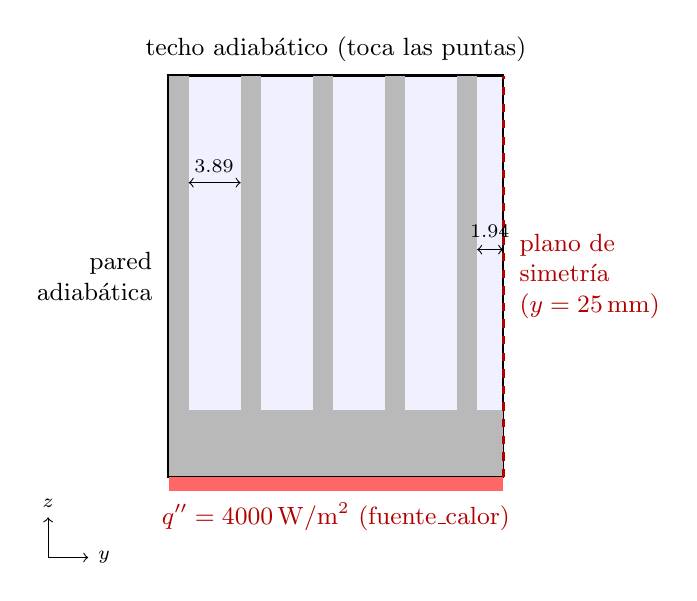
\begin{tikzpicture}[scale=0.17]
\fill[blue!6] (0,0) rectangle (25,30);
\draw[thick] (0,0) rectangle (25,30);
\fill[gray!55] (0,0) rectangle (25,5);
\foreach \i in {0,...,4} {\fill[gray!55] ({\i*5.389},5) rectangle ({\i*5.389+1.5},30);}
\draw[thick] (0,0) -- (25,0);
\draw[very thick,dashed,red!70!black] (25,0) -- (25,30);
\node[right,red!70!black,font=\small,align=left] at (25.5,15) {plano de\\simetría\\($y=\SI{25}{mm}$)};
\node[left,font=\small,align=right] at (-0.5,15) {pared\\adiabática};
\node[above,font=\small] at (12.5,30.3) {techo adiabático (toca las puntas)};
\fill[red!60] (0,-1) rectangle (25,0);
\node[below,font=\small,red!70!black] at (12.5,-1.2) {$q''=\SI{4000}{W/m^2}$ (fuente\_calor)};
\draw[<->] (23.056,17) -- (25,17); \node[above,font=\scriptsize] at (24.0,17.2) {1.94};
\draw[<->] (1.5,22) -- (5.389,22); \node[above,font=\scriptsize] at (3.4,22) {3.89};
\draw[->] (-9,-6) -- (-6,-6) node[right,font=\scriptsize]{$y$}; \draw[->] (-9,-6) -- (-9,-3) node[above,font=\scriptsize]{$z$};
\end{tikzpicture}
\caption{Sección transversal del medio modelo (cotas en mm). Gris: aluminio; azul: aire. El flujo entra perpendicular al papel ($+x$).}
\label{fig:seccion}
\end{figure}

\subsection{Física y condiciones de frontera}
\begin{itemize}
\item \textbf{Régimen laminar y estacionario.} El número de Reynolds basado en el diámetro hidráulico del canal, $D_h=2sH/(s+H)=\SI{6.7}{mm}$, es $\text{Re}_{D_h}\approx\num{1400}$, por debajo de la transición (${\sim}\num{2300}$).
\item \textbf{Transferencia de calor conjugada.} Se resuelve la conducción en el aluminio y la convección en el aire al mismo tiempo. Gracias a la topología compartida de la geometría, la interfaz aire--aluminio es una pared acoplada (\emph{coupled}) con continuidad de temperatura y de flujo de calor.
\item \textbf{Condiciones:} \emph{velocity-inlet} de \SI{2}{m/s} y \SI{298.15}{K}; \emph{pressure-outlet} a 0 Pa manométricos; simetría en $y=\SI{25}{mm}$ (aire y costado de la base); flujo de calor de \SI{4000}{W/m^2} en la cara inferior de la base; las demás paredes del ducto son adiabáticas.
\item \textbf{Solver:} acoplado de presión--velocidad, segundo orden para presión, momento y energía, en doble precisión. Se usaron 500 iteraciones con criterios de residuales de $10^{-5}$ (flujo) y $10^{-8}$ (energía), y la convergencia se confirmó con monitores de $T_{\text{máx}}$ en la base y de presión en la entrada, además de los balances de masa y energía.
\end{itemize}

\subsection{Malla}
Se usaron tetraedros con 5 capas de prismas de inflación en las paredes (crecimiento 1.2), un tamaño global para el ducto y un tamaño más fino para el aluminio, de modo que el canal de \SI{3.9}{mm} quede bien resuelto (Fig.~\ref{fig:malla}).
\begin{figure}[H]
\centering
\includegraphics[width=0.75\linewidth]{img/malla_fina.png}
\caption{Malla fina (\num{608180} elementos): refinamiento alrededor del disipador y transición al ducto.}
\label{fig:malla}
\end{figure}

\section{Independencia de malla}
\begin{table}[H]
\centering
\caption{Mallas y resultados. El balance de energía compara el calor que sale por la salida con los \SI{5}{W} que entran en el medio modelo.}
\label{tab:mallas}
\begin{tabular}{lccrrcccc}\toprule
Malla & $h_{\text{global}}$ & $h_{\text{Al}}$ & Celdas & Nodos & Skew.\ máx. & $R_{th}$ [K/W] & $\Delta p$ [Pa] & Balance E\\\midrule
Gruesa & 6.0 & 1.4 & \num{121992} & \num{62158} & 0.94 & 1.2262 & 9.615 & \SI{0.04}{\%}\\
Intermedia & 4.2 & 1.0 & \num{273504} & \num{131357} & 0.90 & 1.2268 & 8.958 & \SI{0.19}{\%}\\
Fina & 3.0 & 0.7 & \num{608180} & \num{278155} & 0.86 & 1.2315 & 8.890 & \SI{0.11}{\%}\\\bottomrule
\end{tabular}
\end{table}

\begin{figure}[H]
\centering
\includegraphics[width=\linewidth]{img/independencia_malla.png}
\caption{Resistencia térmica y caída de presión contra el número de celdas. Línea discontinua: valor extrapolado de Richardson.}
\label{fig:indep}
\end{figure}

\paragraph{Lectura de la tabla.} $R_{th}$ cambia apenas \SI{0.05}{\%} de la malla gruesa a la intermedia y \SI{0.4}{\%} de la intermedia a la fina: con cinco veces más celdas la resistencia térmica prácticamente no se mueve. La caída de presión es más sensible ($-7.3\,\%$ y luego $-0.8\,\%$) porque depende del gradiente de velocidad en las paredes, que la malla gruesa resuelve peor. En la malla gruesa Fluent reportó flujo inverso en \SI{0.6}{\%} del área de la salida, por la estela del disipador; desaparece al refinar.

\paragraph{GCI.} Con el procedimiento de Celik et al.\ \cite{celik} y razones de refinamiento $r=(N_{i+1}/N_i)^{1/3}\approx1.31$, el orden observado sale $p\approx8$, que no es físico para un esquema de segundo orden. Esto ocurre porque el mallador no genera mallas geométricamente semejantes y porque las diferencias en temperatura ya son del orden del ruido ($\sim\!\SI{0.01}{K}$). En ese caso se recomienda acotar $p$ al orden teórico \cite{roache}. Con $p=2$ y $F_s=1.25$:
\begin{equation}
\text{GCI}_{\text{fina}}=\frac{F_s\,|\varepsilon_{21}|}{r^p-1}:\qquad
\text{GCI}_{R_{th}}=\frac{1.25\times0.0038}{1.305^2-1}=\SI{0.7}{\%},\qquad
\text{GCI}_{\Delta p}=\frac{1.25\times0.0077}{1.305^2-1}=\SI{1.4}{\%}.
\end{equation}
Con el mismo $p=2$, la extrapolación de Richardson da $R_{th}\to\SI{1.238}{K/W}$ y $\Delta p\to\SI{8.79}{Pa}$, a \SI{0.5}{\%} y \SI{1.1}{\%} de la malla fina, dentro de su GCI. La malla fina es la que se usa para el resto del análisis. Estos cálculos y la Fig.~\ref{fig:indep} los genera el script \texttt{analisis\_independencia.py} a partir del archivo CSV de resultados.

\section{Resultados}
\begin{figure}[H]
\centering
\includegraphics[width=0.85\linewidth]{img/escena_disipador_n.png}
\caption{Líneas de corriente coloreadas por temperatura (escala izquierda, 298--\SI{302}{K}) y temperatura superficial del disipador (escala derecha). Disipador completo reconstruido por espejo en el plano de simetría. El aire entra frío, se calienta al pasar por los canales y sale con una estela tibia.}
\label{fig:escena}
\end{figure}

\begin{figure}[H]
\centering
\begin{subfigure}{\linewidth}\centering\includegraphics[width=0.92\linewidth]{img/temp_aire_n.png}\caption{Temperatura [K].}\end{subfigure}\\[4pt]
\begin{subfigure}{\linewidth}\centering\includegraphics[width=0.92\linewidth]{img/vel_aire_n.png}\caption{Magnitud de velocidad [m/s].}\end{subfigure}
\caption{Plano horizontal a media altura de las aletas ($z=\SI{17.5}{mm}$), con el flujo de izquierda a derecha; las 10 aletas se muestran por espejo del medio modelo.}
\label{fig:plano}
\end{figure}

\begin{figure}[H]
\centering
\includegraphics[width=0.75\linewidth]{img/temp_disipador_n.png}
\caption{Temperatura superficial del disipador completo (espejo del medio modelo), de \SI{308.9}{K} en el borde de ataque de las puntas a \SI{310.5}{K} en la base.}
\label{fig:tdisip}
\end{figure}

\paragraph{Campo térmico.} Todo el disipador está dentro de un rango de solo \SI{1.6}{K} (Fig.~\ref{fig:tdisip}): el aluminio conduce tan bien que las aletas quedan casi a la temperatura de la base, en acuerdo con $\eta_f\approx0.96$. La zona más fría es el borde de ataque de las puntas, donde la capa límite es más delgada y el aire llega más frío. En el plano medio (Fig.~\ref{fig:plano}a) se ve crecer la capa límite térmica a lo largo de cada canal; a la salida el aire se mezcla en una estela cuyo aumento promedio de temperatura es $\Delta T_b=Q/(\dot m c_p)=5/(0.001746\times1007)=\SI{2.8}{K}$.

\paragraph{Campo de velocidad.} El aire llega a \SI{2}{m/s} y dentro de los canales alcanza hasta \SI{5}{m/s} en el centro (Fig.~\ref{fig:plano}b). La velocidad \emph{media} en el canal es \SI{3.43}{m/s}; el máximo es mayor porque el perfil laminar es cero en las paredes y máximo al centro. Detrás del disipador los chorros de cada canal se mezclan.

\paragraph{Balances.} El flujo másico en la entrada es $\dot m=\SI{1.7460e-3}{kg/s}$, que coincide exactamente con $\rho U_\infty A$, y el de la salida difiere en \SI{0.03}{\%}. En energía, de los \SI{5.000}{W} aplicados salen \SI{4.994}{W} por la salida (\SI{0.11}{\%}).

\section{Validación}
\begin{table}[H]
\centering
\caption{Comparación de la resistencia térmica.}
\label{tab:valid}
\begin{tabular}{lccc}\toprule
Fuente & $R_{th}$ [K/W] & $T_{\text{base}}$ [\si{\celsius}] & CFD vs.\ fuente\\\midrule
Correlación (A): $U_c=\SI{2.86}{m/s}$ & 1.306 & 38.1 & $-5.7\,\%$\\
Correlación (B): $U_c=\SI{3.43}{m/s}$ & 1.197 & 37.0 & $+2.9\,\%$\\
\textbf{CFD, malla fina} & \textbf{1.232} & \textbf{37.3} & ---\\\bottomrule
\end{tabular}
\end{table}

El resultado CFD cae dentro de la banda que definen las dos estimaciones analíticas (Tabla~\ref{tab:valid}). Las diferencias, de $-6$ y $+3\,\%$, son entre 4 y 8 veces mayores que la incertidumbre numérica (GCI de \SI{0.7}{\%}), así que no vienen de la malla sino de las simplificaciones de la correlación:
\begin{itemize}
\item La correlación de placa plana supone capas límite independientes, pero en este canal se juntan antes del final de la aleta ($\delta>s/2$). Al juntarse, el gradiente de temperatura en la pared baja y el coeficiente real es menor que el de placa plana, lo que empuja $R_{th}$ hacia arriba respecto al caso (B).
\item La correlación usa un $\bar h$ uniforme. En el CFD el coeficiente es mayor en el borde de ataque y en las puntas, y el aire se calienta conforme avanza por el canal, lo que reduce la diferencia de temperatura disponible al final de la aleta.
\item La elección de la velocidad característica (A o B) cambia la estimación en \SI{9}{\%}. Esa sola elección es mayor que la discrepancia con el CFD, y muestra el valor de resolver el flujo real en vez de suponerlo.
\end{itemize}

\section{Herramientas y flujo de trabajo}
\begin{itemize}
\item \textbf{Ansys SpaceClaim} (geometría paramétrica por script en Python/IronPython), \textbf{Ansys Meshing} y \textbf{Ansys Fluent 2026~R1 Student}.
\item \textbf{Python} (NumPy, Matplotlib) para la parte que no es CFD:
  \begin{itemize}
  \item \texttt{referencia\_disipador.py}: correlación de placa plana, eficiencia de aleta y $R_{th}$ para los dos casos de velocidad (Código~\ref{lst:ref}).
  \item \texttt{analisis\_independencia.py}: lee las tres mallas desde \texttt{independencia\_malla.csv}, calcula el orden observado, la extrapolación de Richardson y el GCI, y genera la Fig.~\ref{fig:indep} (Código~\ref{lst:gci}).
  \end{itemize}
\item Los valores finales de cada malla se tomaron de los archivos de monitores de Fluent (\texttt{*-rfile.out}), no de la pantalla, para conservar todas las cifras.
\end{itemize}

\section{Conclusiones}
\begin{itemize}
\item El disipador tiene una resistencia térmica de $R_{th}=\SI{1.23}{K/W}$: con \SI{10}{W} la base llega a \SI{37.3}{\celsius} con aire a \SI{25}{\celsius}. La caída de presión del aire es de \SI{8.9}{Pa}.
\item La solución es independiente de la malla: la incertidumbre numérica (GCI) es de \SI{0.7}{\%} en $R_{th}$ y \SI{1.4}{\%} en $\Delta p$, y los balances de masa y energía cierran con errores menores a \SI{0.2}{\%}.
\item El resultado queda entre las dos estimaciones con correlaciones clásicas ($-6$ y $+3\,\%$). La diferencia se explica por la interacción de las capas límite en canales angostos, que las correlaciones de placa plana no capturan.
\item La eficiencia de aleta es alta (las aletas solo están \SI{1.6}{K} más frías que la base), así que agregar altura de aleta rendiría poco. Para mejorar el diseño convendría más bien aumentar el número de aletas o la velocidad del aire, buscando el compromiso con la caída de presión.
\end{itemize}

\begin{thebibliography}{9}
\bibitem{incropera} T.~L.~Bergman, A.~S.~Lavine, F.~P.~Incropera y D.~P.~DeWitt, \emph{Fundamentals of Heat and Mass Transfer}, 8a ed., Wiley, 2018.
\bibitem{celik} I.~B.~Celik, U.~Ghia, P.~J.~Roache, C.~J.~Freitas, H.~Coleman y P.~E.~Raad, ``Procedure for estimation and reporting of uncertainty due to discretization in CFD applications'', \emph{Journal of Fluids Engineering}, 130(7), 078001, 2008.
\bibitem{roache} P.~J.~Roache, \emph{Verification and Validation in Computational Science and Engineering}, Hermosa Publishers, 1998.
\end{thebibliography}
\appendix
\section{Fragmentos de código}
\label{ap:codigo}
Se muestran solo las funciones centrales; los scripts completos están en la carpeta \texttt{validacion/} del proyecto.
\lstinputlisting[firstline=27,lastline=41,firstnumber=27,caption={\texttt{referencia\_disipador.py}: $R_{th}$ con placa plana y eficiencia de aleta.},label=lst:ref]{code/referencia_disipador.py}
\lstinputlisting[firstline=24,lastline=38,firstnumber=24,caption={\texttt{analisis\_independencia.py}: orden observado, Richardson y GCI.},label=lst:gci]{code/analisis_independencia.py}
\end{document}
